\subsubsection{Methodology.}
Decision Tree is a rule-based machine learning algorithm, where its set of rules is generated by recursively splitting the dataset on a chosen feature so that the separation maximises a certain target criterion (e.g. entropy gain, Gini impurity, etc.). Despite being generally less accurate comparing to other machine learning models, it rises in terms of comprehensibility and explainability. As the algorithm does not assume the underlying distribution of the data, transformation such as standardisation or Box-Cox are not required at this stage.

\subsubsection{Experiments \& Results.}
Experiments focus in finding the best splitting algorithm, that includes the criterion to be optimised for splitting and the terminating condition. In other words, the following parameters are tested:

\begin{itemize}
    \item \textbf{\texttt{minsplit}}. Number of elements in a leaf node, where the algorithm stops splitting. \texttt{minsplit} is let to be \( 5, 10, 15, \cdots, 100 \);
    \item \textbf{\texttt{split}}. Algorithm to determine the optimal split. Either 'Information gain' (Entropy gain) or 'Gini impurity'.
\end{itemize}

In terms of sensitivity at \( \delta = 0.5 \), entropy-based algorithms fit well for a low \texttt{minsplit}, but as \texttt{minsplit} increases, its performance stagnated, both in the full or simplified tree. In contrast, Gini-based trees underperform with low values of \texttt{minsplit}, but gradually improve when \texttt{minsplit} increases. There is also an observation that simplifing the input does not change the metrics for large \texttt{minsplit}s, suggesting the possibility that the algorithm abandons these uncorrelated features at its internal procedures.

\begin{figure}[h]
    \centering
    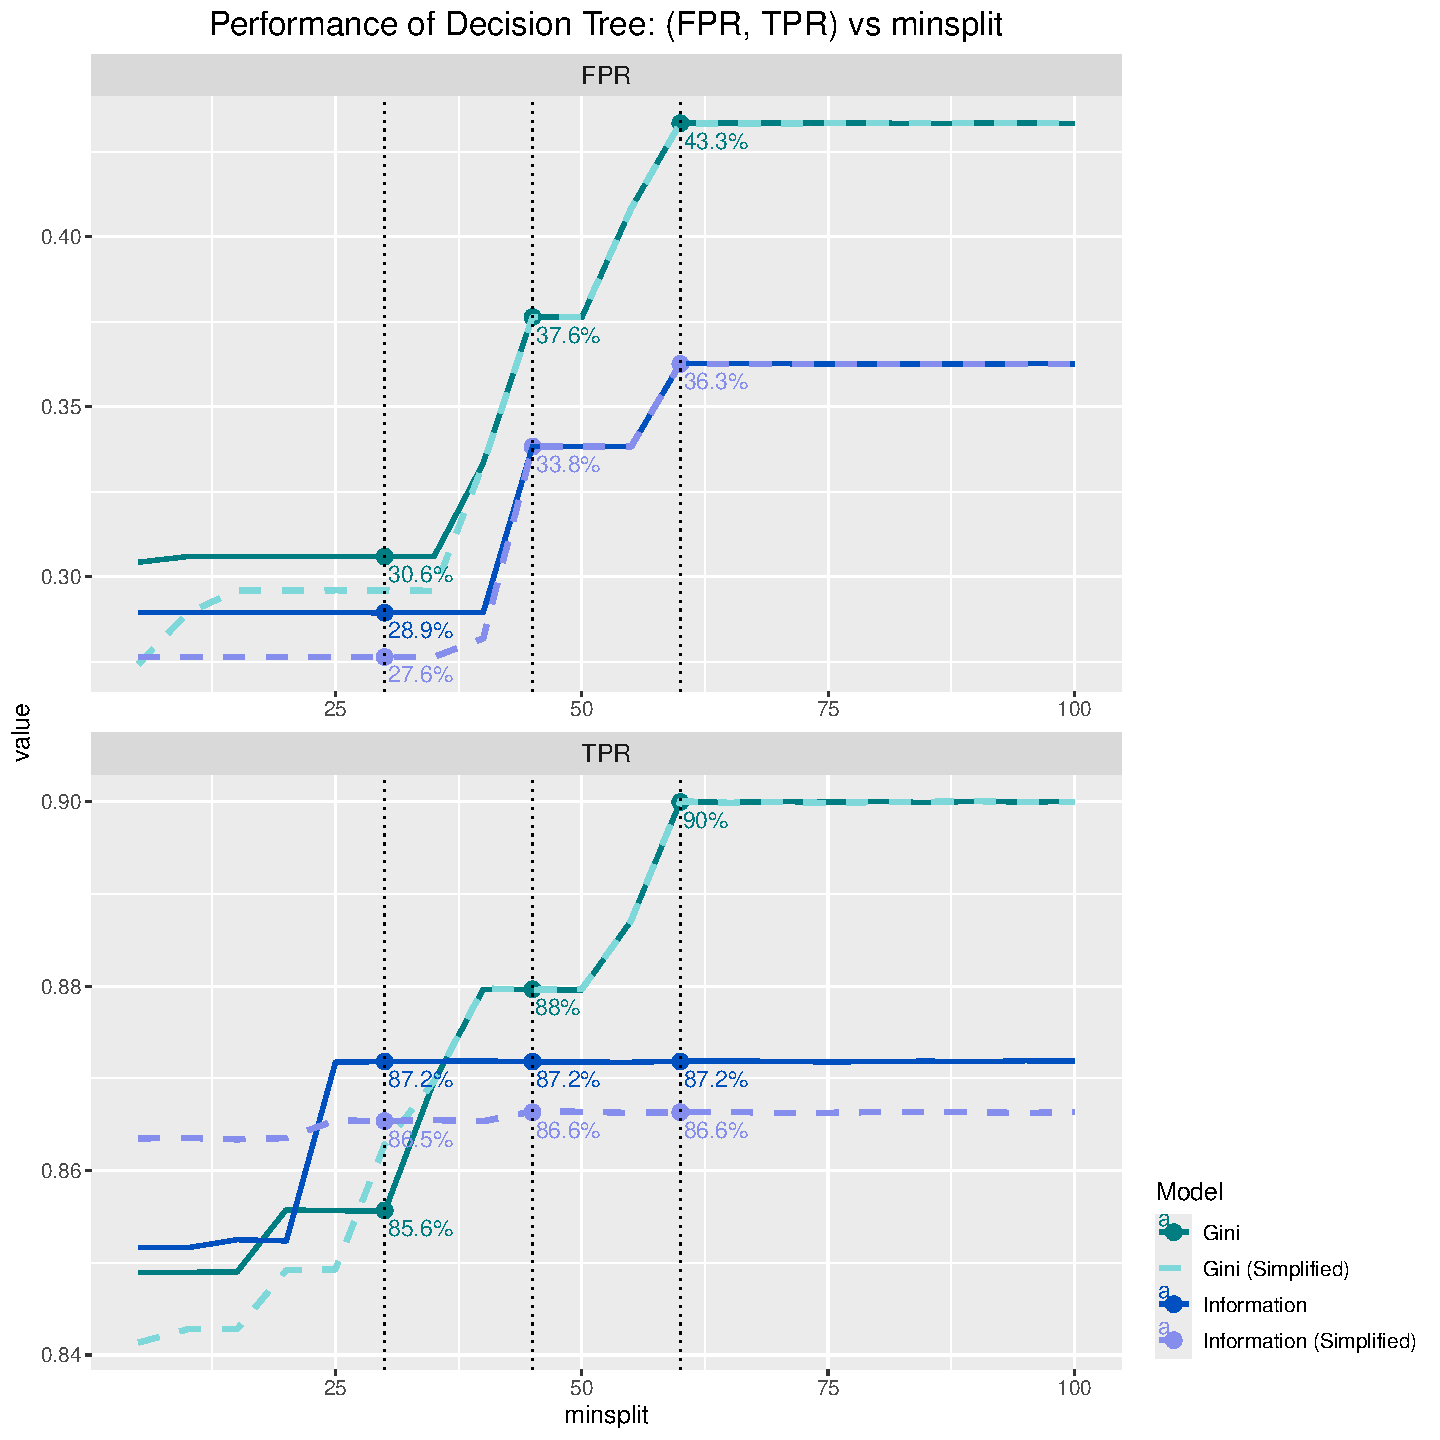
\includegraphics[width=\linewidth]{32.DecisionTree.pdf}
    \caption{\centering TPR/FPR performance of decision trees vs. minsplit}
\end{figure}

One should be cautious, however, when setting a high value of \texttt{minsplit}, as it would result in an underfitting tree with most of the datapoint classified as True, optimising TPR at the cost of a high False Positive Rate (FPR). In this example, although a decision tree with \( \texttt{minsplit} = 60 \) produces a \( 90.0\% \) sensitivity, its speficitivity is a very impractical \( 43.3\% \). The tree structure is a simple \( 2 \)-layer tree that relies only on \texttt{blood.disorder} and \texttt{chest.pain}, hence the underfitting phenomenon.

\begin{figure}[h]
    \centering
    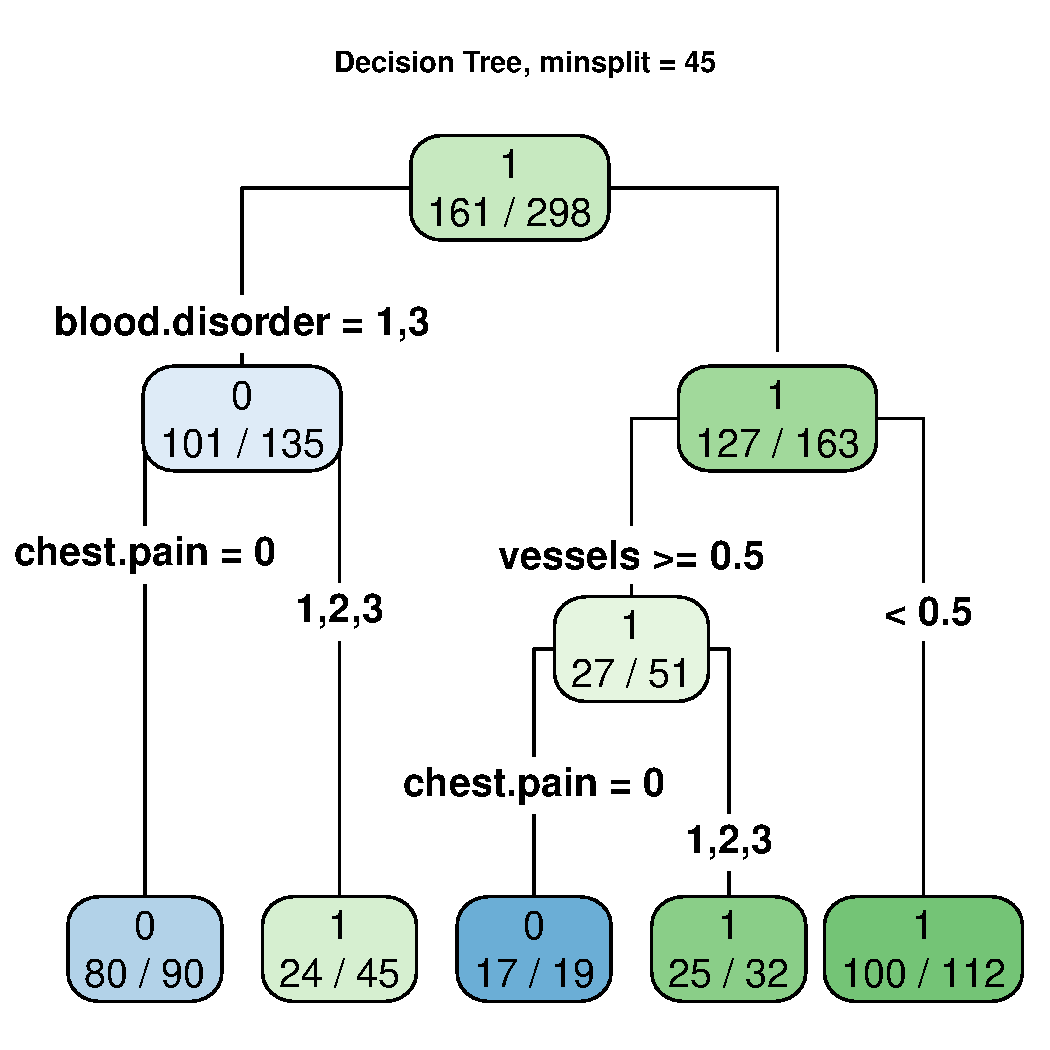
\includegraphics[width=0.45\linewidth]{32.DecisionTree-45.pdf}
    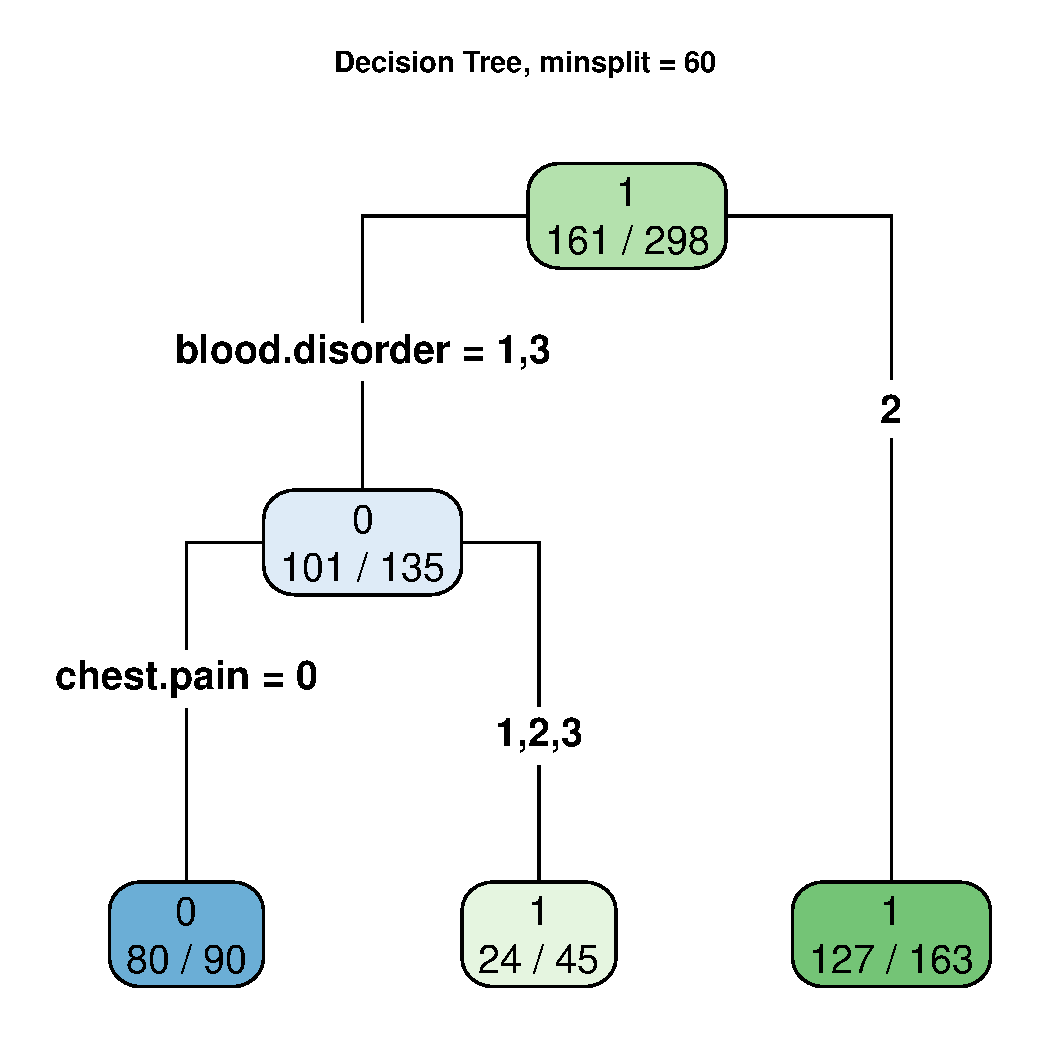
\includegraphics[width=0.45\linewidth]{32.DecisionTree-60.pdf}
    \caption{\centering Left: Moderate 45-minsplit decision tree; Right: Underfitting 60-minsplit decision tree}
\end{figure}

Choosing the 'best' model amongst all decision trees is rather a nuanced task due to the complex relationship between the \texttt{minsplit} hyperparameter with TPR-FPR metrics. For now, these two decision trees are left for further investigation:
\begin{itemize}
    \item \textbf{Information gain, \( \texttt{minsplit} = 30 \)}
    \item \textbf{Gini, \( \texttt{minsplit} = 45 \)}
\end{itemize}
